\documentclass[lettersize,journal]{IEEEtran}
\usepackage{amsmath,amsfonts}
\usepackage{algorithmic}
\usepackage{array}
\usepackage[caption=false,font=normalsize,labelfont=sf,textfont=sf]{subfig}
\usepackage{textcomp}
\usepackage{stfloats}
\usepackage{url}
\usepackage{verbatim}
\usepackage{graphicx}

\usepackage{enumitem} % 用于自定义列表样式
\usepackage{amsmath}  % 用于数学符号和环境
\hyphenation{op-tical net-works semi-conduc-tor IEEE-Xplore}
\def\BibTeX{{\rm B\kern-.05em{\sc i\kern-.025em b}\kern-.08em
    T\kern-.1667em\lower.7ex\hbox{E}\kern-.125emX}}
\usepackage{balance}
\begin{document}
\title{Formal language and automatonics assignment}
\author{Junqi Jing-2311104-2023210913
\thanks{}}

\markboth{Journal of \LaTeX\ Class Files,~Vol.~18, No.~9, September~2020}%
{How to Use the IEEEtran \LaTeX \ Templates}

\maketitle

\section{\textbf{Why a regular language is called "regular"?}}
In this section, you can introduce the concept of a regular language. Discuss its significance in formal language theory and why it is essential to classify languages based on their computational properties.

\subsection*{1. Regular Expressions}

In this section, you need to explain what a regular expression is. You can consider:
- The definition and purpose of regular expressions.
- Describe common operations used in regular expressions, such as:

\begin{itemize}
    \item **Concatenation**: Explain how strings can be joined together.
    \item **Union (alternation)**: Indicate how to represent choices between different expressions.
    \item **Kleene star**: Discuss the concept of repetition in expressions.
\end{itemize}

Provide insights into how these operations work together to define languages concisely.
\subsection*{2. Finite Automata}

In this section, describe finite automata as a computational model. You should cover:
- The definition of finite automata and their function in recognizing regular languages.
- Different types of finite automata, such as:
  - **Deterministic Finite Automata (DFA)**: Explain how they function with unique state transitions.
  - **Non-Deterministic Finite Automata (NFA)**: Describe how they can have multiple possible transitions for a given state and input.

Highlight how both types can effectively recognize the same class of languages.
\subsection*{3. Closure Properties}

Here, outline the closure properties of regular languages. Discuss:
- What closure properties are and their significance in language theory.
- List and explain the operations under which regular languages are closed, such as:
\begin{itemize}
    \item **Union**: Describe how combining languages retains regularity.
    \item **Concatenation**: Explain how joining two regular languages results in another regular language.
    \item **Kleene star**: Discuss the implications of allowing repetition.
    \item **Intersection**: Explore how the intersection of two regular languages is still regular.
    \item **Complementation**: Describe how taking the complement of a regular language yields another regular language.
\end{itemize}

Explain how these properties contribute to the understanding of regular languages.

\subsection*{4. Historical Context}

In this section, provide a brief historical overview. Discuss:
- The introduction of the term "regular" and its significance in the field.
- Mention key figures, such as **Stephen Kleene**, and their contributions to formalizing regular languages.

This context can help frame the importance of regular languages in the development of computer science and linguistics.

\subsection*{Conclusion}

Summarize the key points made throughout the document. Reflect on:
- Why regular languages are foundational in computer science.
- Their predictability and simplicity compared to other language classes, emphasizing their role in formal language theory.


\section{\textbf{HW3}}
\begin{figure}[h]  
    \centering
    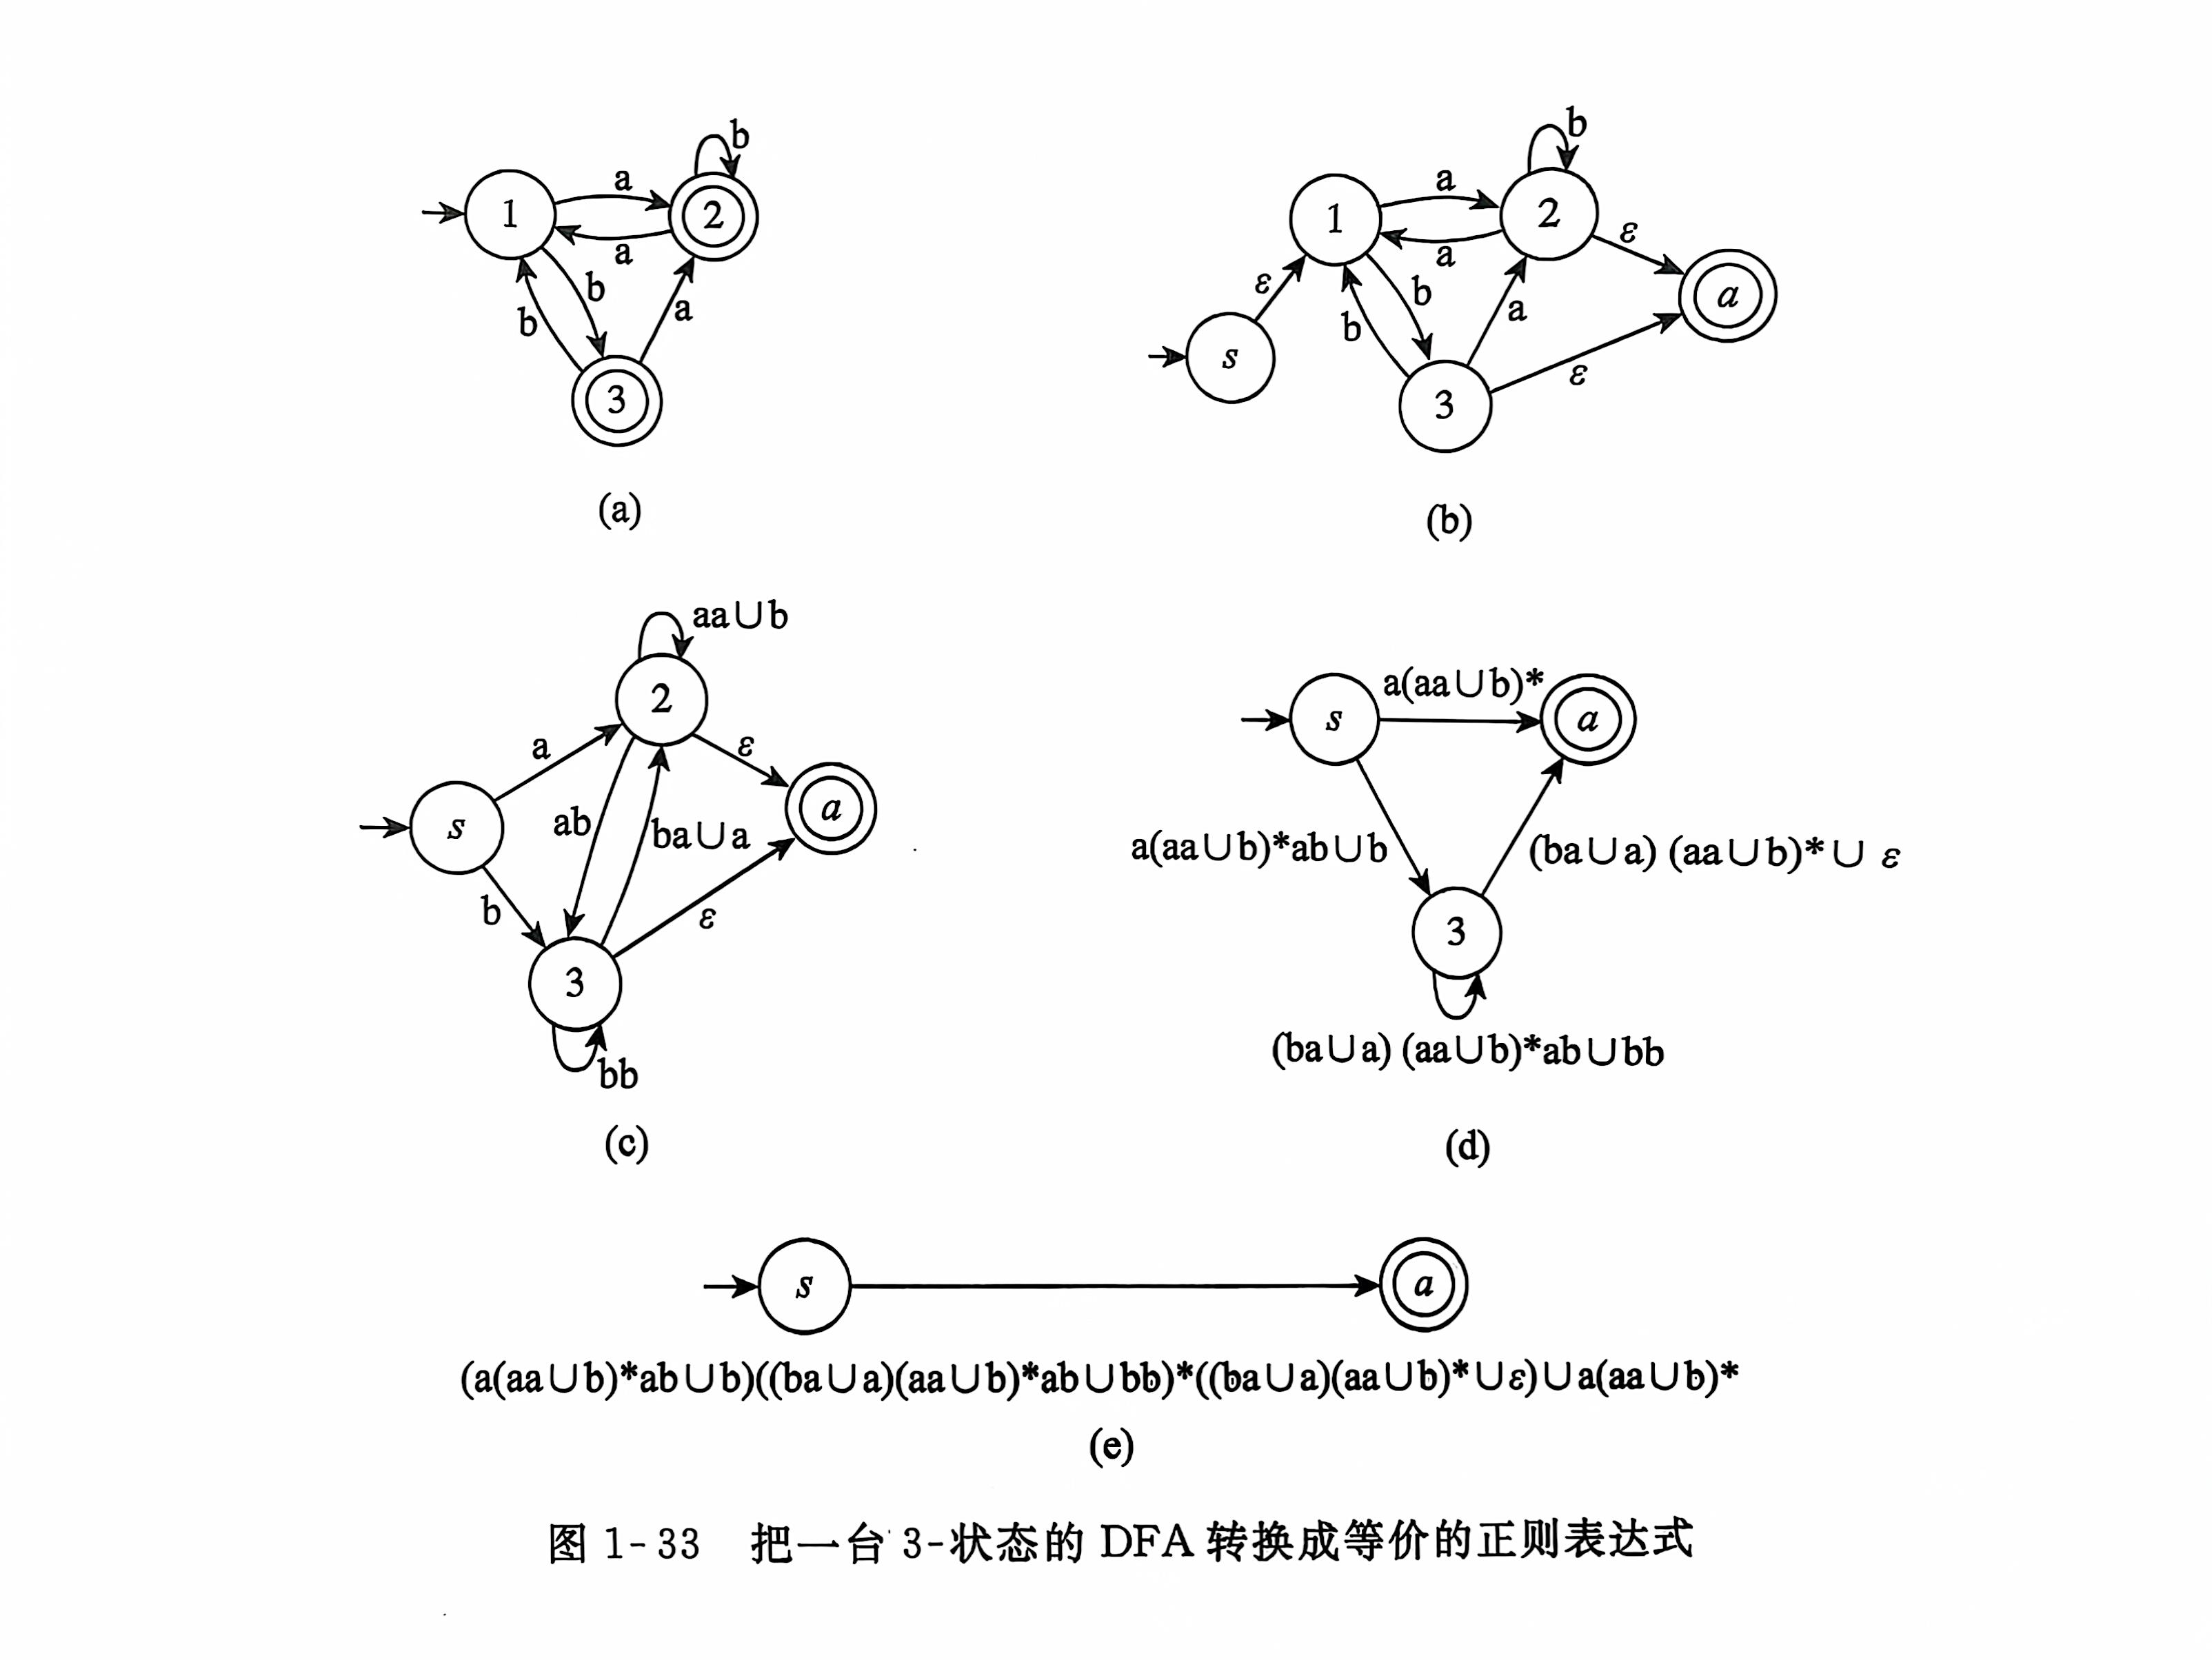
\includegraphics[width=0.5\textwidth]{hw3.jpg} 
    \caption{Converting a 3-state DFA into an equivalent regular expression}
    \label{fig:hw3}
\end{figure}
\subsection*{Guiding Thoughts for DFA Analysis}

\begin{enumerate}[label=\arabic*.] 
    \item \textbf{Identify States and Transitions}: 
    Examine the states in the DFA and the corresponding transitions between them. Consider the symbols that trigger transitions between states. This will give you a clear understanding of the automaton's structure.
    
    \item \textbf{$\varepsilon$-Closure}: 
    Determine how to handle $\varepsilon$-transitions. Analyze how you can compute the $\varepsilon$-closure for states with $\varepsilon$-transitions, which allows simplification of the automaton by considering reachable states without consuming input symbols.
    
    \item \textbf{Build the Regular Expression}: 
    Based on the transitions and states, derive the regular expression. Start from basic paths, identify loops (if any), and use the Kleene star ($^*$) to represent repeated sequences. Pay attention to how different paths interact.
    
    \item \textbf{Simplify the Regular Expression}: 
    Once you have derived the full regular expression, simplify it by combining equivalent parts and eliminating redundancies. Ensure the expression is as concise and clear as possible, while maintaining equivalence to the DFA.
\end{enumerate}
\section{HW4}
Convert the following \textbf{CFG} (Context-Free Grammar) into an equivalent \textbf{Chomsky Normal Form (CNF)} grammar.
\[
\begin{array}{rcl}
    A & \rightarrow & BAB \ \mid \ B \ \mid \ \varepsilon \\
    B & \rightarrow & 00 \ \mid \ \varepsilon
\end{array}
\]

\subsection*{Guiding Thoughts for Converting CFG to CNF}

\noindent Consider the following steps when converting a \textbf{CFG} to \textbf{CNF}:

\begin{enumerate}[label=\arabic*.] 
    \item \textbf{Eliminate $\varepsilon$-productions}: 
    Identify and eliminate productions that derive the empty string ($\varepsilon$). This involves replacing occurrences of nullable variables with alternative derivations or removing them, ensuring the grammar does not generate $\varepsilon$ unless necessary for the language.
    
    \item \textbf{Eliminate Unit Productions}: 
    Identify and eliminate unit productions, which are rules of the form $A \rightarrow B$ where $A$ and $B$ are non-terminal symbols. Replace them with the productions of $B$. This step ensures that all productions either have terminals or combinations of terminals and non-terminals.

    \item \textbf{Convert Productions to Binary Form}: 
    Convert all productions into binary form, where each rule's right-hand side contains at most two non-terminals or one terminal symbol. For any production with more than two symbols, introduce additional intermediate variables. For instance, a rule like $A \rightarrow XYZ$ would be converted into two rules, such as $A \rightarrow XZ_1$ and $Z_1 \rightarrow YZ$.
\end{enumerate}


\end{document}


